% ---------------------------- Problem 1----------------------------------
\subsubsection*{\center Задача № 1.}
{\bf Условие.~}
Найти область определения функции
$$
y(x) = \lg\biggl(\dfrac{x+4}{1-2x}\biggr).
$$	
{\bf Решение.~}	
$D_f: \dfrac{x+4}{1-2x}>0 \Leftrightarrow x \in (-4;\,-1/2).$

% ---------------------------- Problem 2----------------------------------
\subsubsection*{\center Задача № 2.}
{\bf Условие.~}
Исследовать функцию на чётность и нечётность
$$
y(x) = \ctg(\cos(\tg(x))).
$$	
{\bf Решение.~}	
$$
y(-x) = \ctg(\cos(\tg(-x))) = \ctg(\cos(-\tg(x))) = \ctg(\cos(\tg(x))) = y(x).
$$	
Отсюда, $y(x)$ --- чётная функция.


% ---------------------------- Problem 3----------------------------------
\subsubsection*{\center Задача № 3.}
{\bf Условие.~}
Используя элементарные преобразования, построить эскизы графиков функций (а)--(д).
$$
\begin{array}{cc}
\text{3(а):} & y(x) = -1 - \sin(2x + \pi/4), \\
\text{3(б):} & y(x) = |2 \sqrt[3]{x+5} - 1|, \\
\text{3(в):} & y(x) = 1 - \log_3|x+1|, \\
\text{3(г):} & y(x) = \dfrac{1}{3} 2^{2x+1} - \dfrac{4}{3}, \\[8pt]
\text{3(д):} & y(x) = \dfrac{3\pi}{8} + \dfrac{3}{2}\arctg(2x-3).
\end{array}
$$
{\bf Решение.~}
% ---------------- Problem 3а----------------
Последовательность элементарных преобразований графика функции 3(а).
\begin{center}
	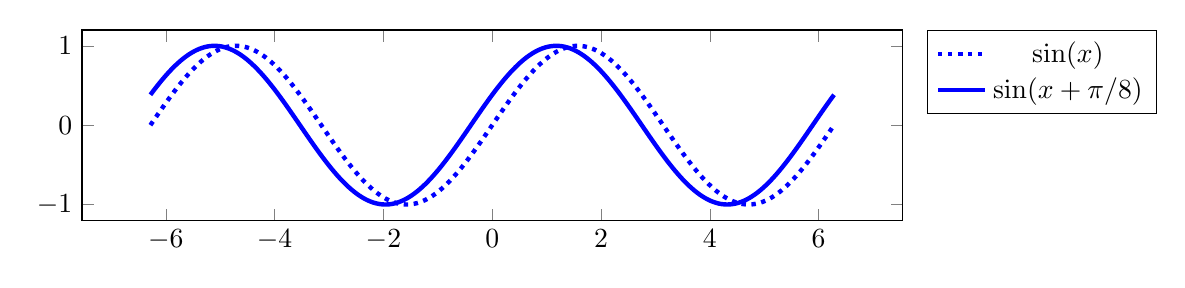
\begin{tikzpicture}
	\begin{axis}[width=12cm, height=4cm, samples=250, domain=-2*pi:2*pi,legend pos=outer north east]
	\addplot[blue, dotted, ultra thick, samples=250, domain=-2*pi:2*pi]{sin(deg(x))};
	\addlegendentry{$\sin(x)$}
	\addplot[blue, ultra thick, samples=250, domain=-2*pi:2*pi]{sin(deg(x+pi/8))};
	\addlegendentry{$\sin(x+\pi/8)$}
	\end{axis}
	\end{tikzpicture}
	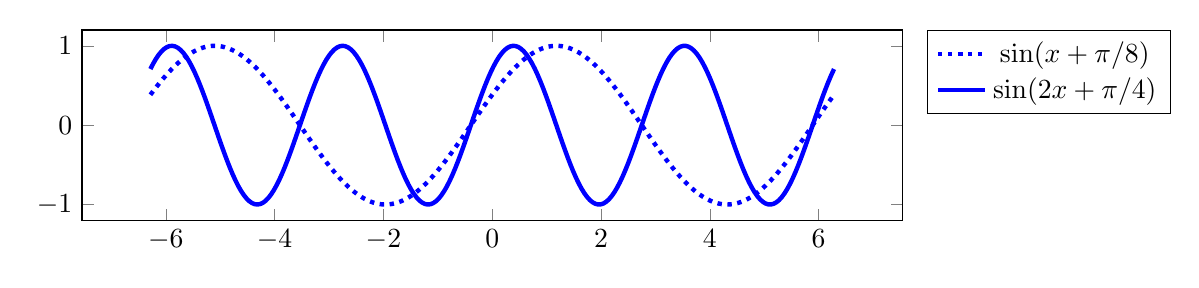
\begin{tikzpicture}
	\begin{axis}[width=12cm, height=4cm, samples=250, domain=-2*pi:2*pi,legend pos=outer north east]
	\addplot[blue, dotted, ultra thick, samples=250, domain=-2*pi:2*pi]{sin(deg(x+pi/8))};
	\addlegendentry{$\sin(x+\pi/8)$}
	\addplot[blue, ultra thick, samples=250, domain=-2*pi:2*pi]{sin(2*deg(x+pi/8))};
	\addlegendentry{$\sin(2x+\pi/4)$}
	\end{axis}
	\end{tikzpicture}
	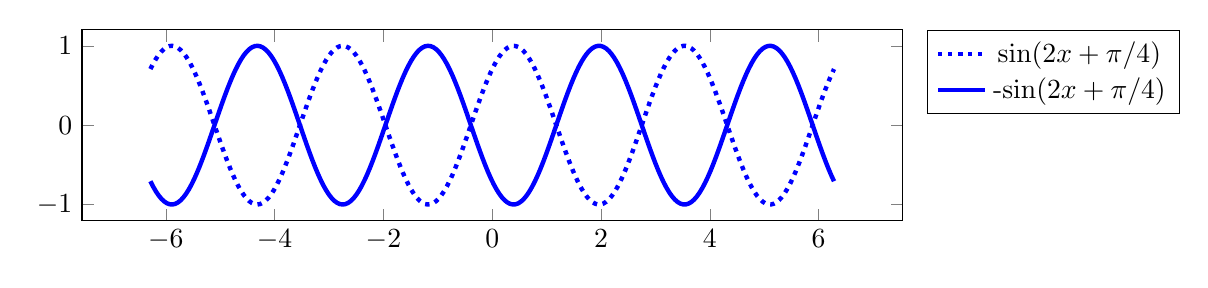
\begin{tikzpicture}
	\begin{axis}[width=12cm, height=4cm, samples=250, domain=-2*pi:2*pi,legend pos=outer north east]
	\addplot[blue, dotted, ultra thick, samples=250, domain=-2*pi:2*pi]{sin(2*deg(x+pi/8))};
	\addlegendentry{$\sin(2x+\pi/4)$}
	\addplot[blue, ultra thick, samples=250, domain=-2*pi:2*pi]{-sin(2*deg(x+pi/8))};
	\addlegendentry{-$\sin(2x+\pi/4)$}
	\end{axis}
	\end{tikzpicture}
	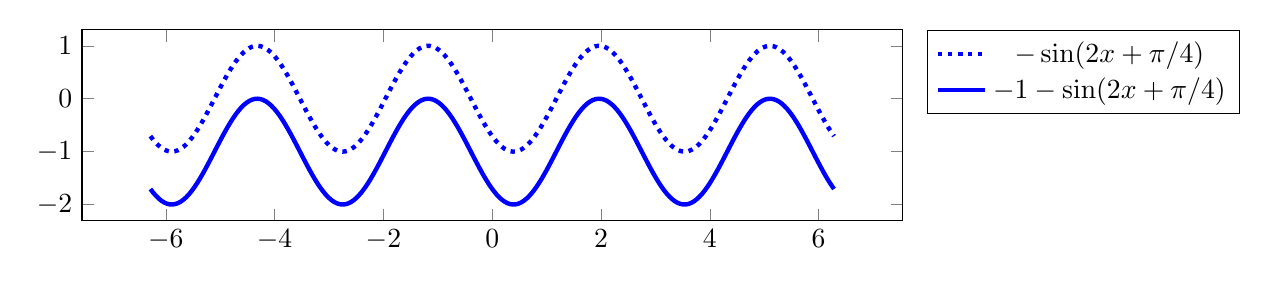
\begin{tikzpicture}
	\begin{axis}[width=12cm, height=4cm, samples=250, domain=-2*pi:2*pi,legend pos=outer north east]
	\addplot[blue, dotted, ultra thick, samples=250, domain=-2*pi:2*pi]{-sin(2*deg(x+pi/8))};
	\addlegendentry{$-\sin(2x+\pi/4)$}
	\addplot[blue, ultra thick, samples=250, domain=-2*pi:2*pi]{-1-sin(2*deg(x+pi/8))};
	\addlegendentry{$-1-\sin(2x+\pi/4)$}
	\end{axis}
	\end{tikzpicture}
\end{center}

% ---------------- Problem 3б----------------
Последовательность элементарных преобразований графика функции 3(б).
\begin{center}
	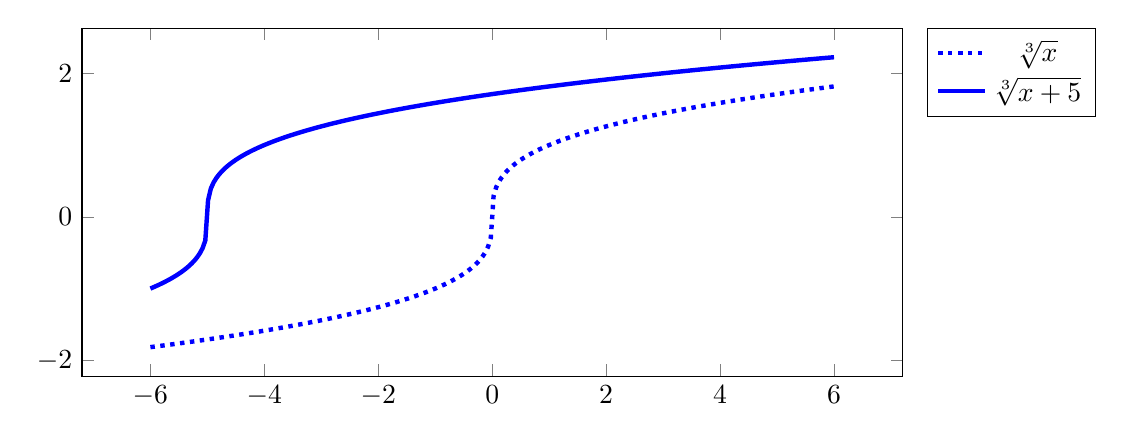
\begin{tikzpicture}
	\begin{axis}[width=12cm, height=6cm, samples=250, domain=-6:6,legend pos=outer north east]
	\addplot[blue, dotted, ultra thick]{sign(x)*abs(x)^(1/3)};
	\addlegendentry{$\sqrt[3]{x}$}
	\addplot[blue, ultra thick]{sign(x+5)*abs(x+5)^(1/3)};
	\addlegendentry{$\sqrt[3]{x+5}$}	
	\end{axis}
	\end{tikzpicture}
	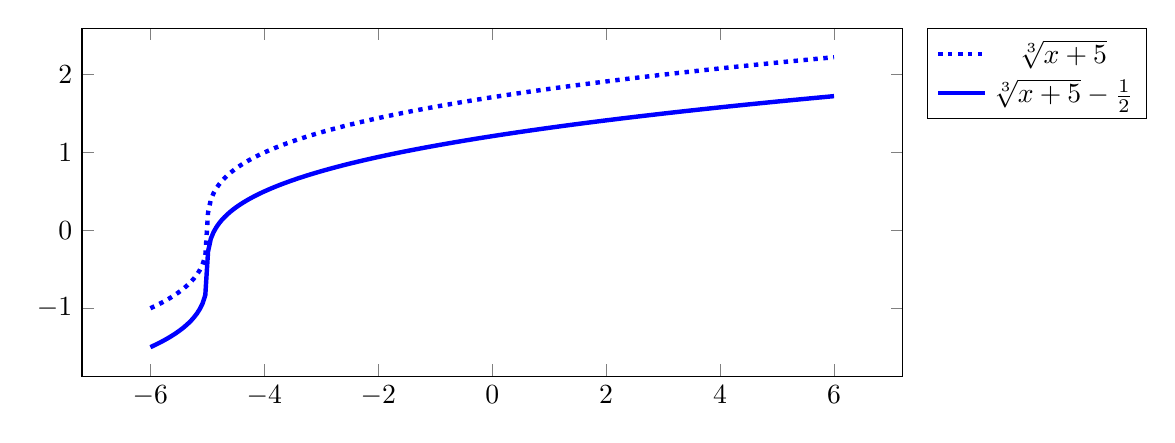
\begin{tikzpicture}
	\begin{axis}[width=12cm, height=6cm, samples=250, domain=-6:6,legend pos=outer north east]
	\addplot[blue, dotted, ultra thick]{sign(x+5)*abs(x+5)^(1/3)};
	\addlegendentry{$\sqrt[3]{x+5}$}	
	\addplot[blue, ultra thick]{sign(x+5)*abs(x+5)^(1/3)-1/2};
	\addlegendentry{$\sqrt[3]{x+5}-\frac12$}
	\end{axis}
	\end{tikzpicture}
	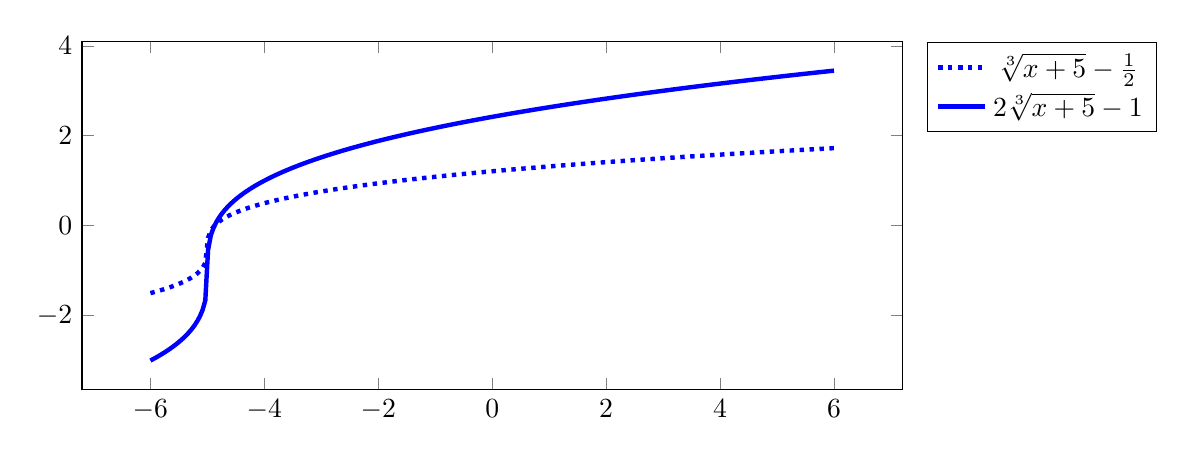
\begin{tikzpicture}
	\begin{axis}[width=12cm, height=6cm, samples=250, domain=-6:6,legend pos=outer north east]
	\addplot[blue, dotted, ultra thick]{sign(x+5)*abs(x+5)^(1/3)-1/2};
	\addlegendentry{$\sqrt[3]{x+5}-\frac12$}
	\addplot[blue, ultra thick]{2*(sign(x+5)*abs(x+5)^(1/3)-1/2)};
	\addlegendentry{$2\sqrt[3]{x+5}-1$}	
	\end{axis}
	\end{tikzpicture}
	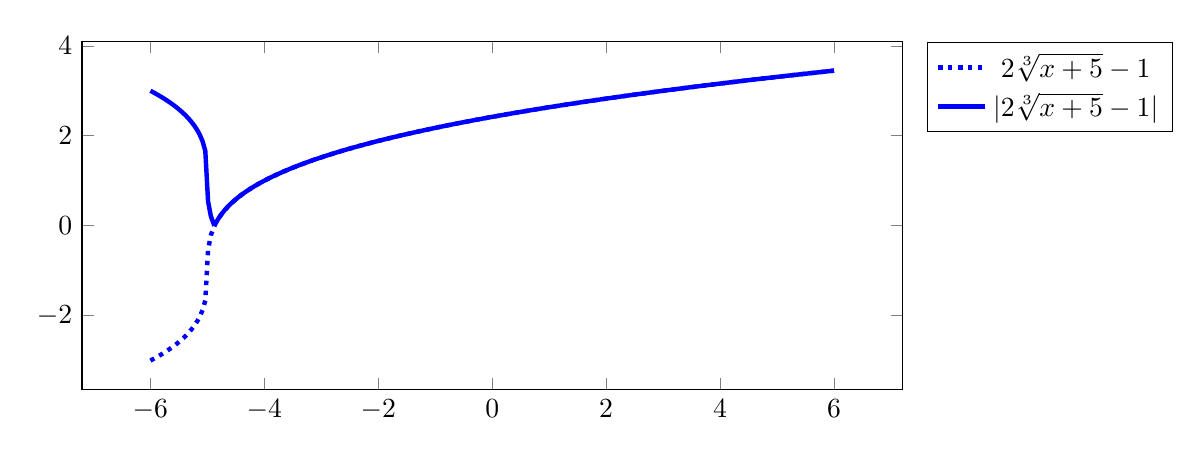
\begin{tikzpicture}
	\begin{axis}[width=12cm, height=6cm, samples=250, domain=-6:6,legend pos=outer north east]
	\addplot[blue, dotted, ultra thick]{2*sign(x+5)*abs(x+5)^(1/3)-1};
	\addlegendentry{$2\sqrt[3]{x+5}-1$}
	\addplot[blue, ultra thick]{abs(2*(sign(x+5)*abs(x+5)^(1/3)-1/2))};
	\addlegendentry{$|2\sqrt[3]{x+5}-1|$}	
	\end{axis}
	\end{tikzpicture}
\end{center}

% ---------------- Problem 3в----------------
Последовательность элементарных преобразований графика функции 3(в).
\begin{center}
	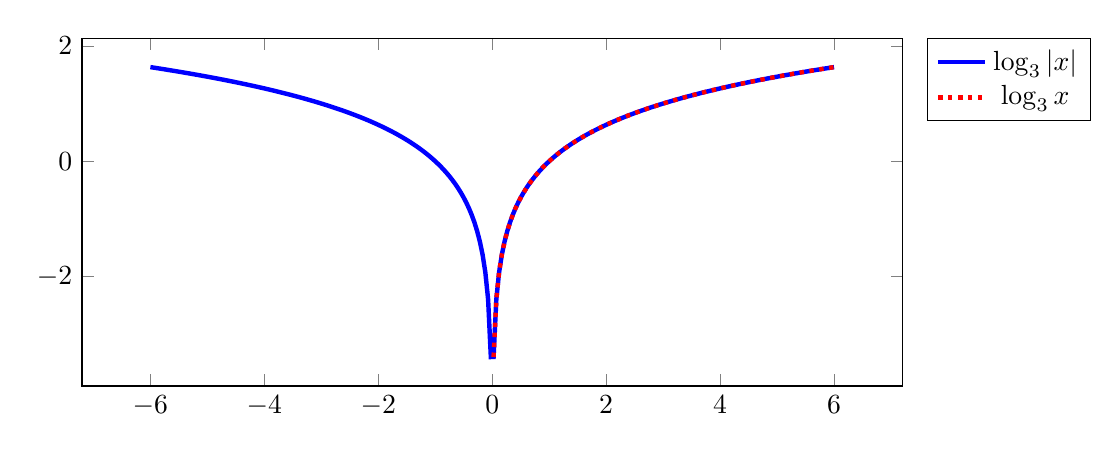
\begin{tikzpicture}
	\begin{axis}[width=12cm, height=6cm, samples=250, domain=-6:6,legend pos=outer north east]
	\addplot[blue, ultra thick]{ln(abs(x))/ln(3)};
	\addlegendentry{$\log_3{|x|}$}	
	\addplot[red, dotted, ultra thick]{ln(x)/ln(3)};
	\addlegendentry{$\log_3{x}$}	
	\end{axis}
	\end{tikzpicture}
	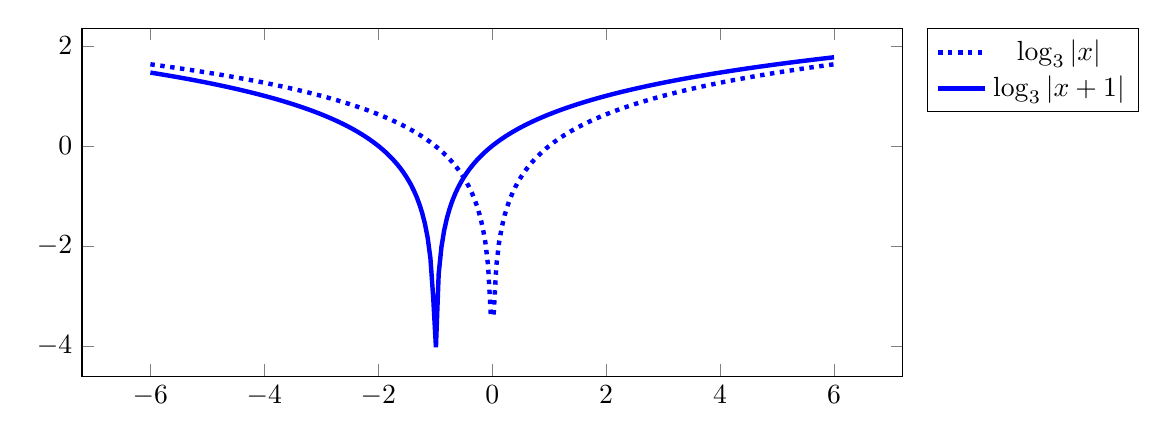
\begin{tikzpicture}
	\begin{axis}[width=12cm, height=6cm, samples=250, domain=-6:6,legend pos=outer north east]
	\addplot[blue, dotted, ultra thick]{ln(abs(x))/ln(3)};
	\addlegendentry{$\log_3{|x|}$}	
	\addplot[blue, ultra thick]{ln(abs(x+1))/ln(3)};
	\addlegendentry{$\log_3{|x+1|}$}	
	\end{axis}
	\end{tikzpicture}
	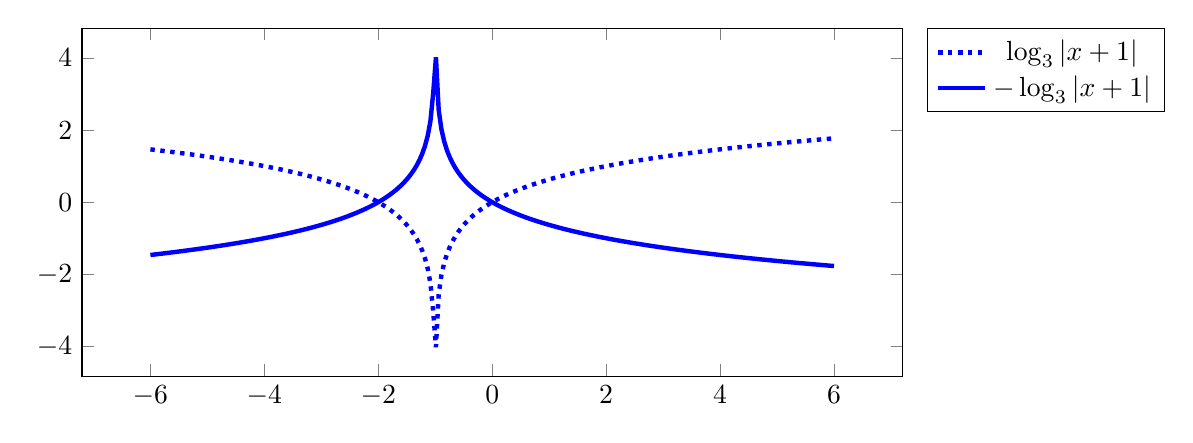
\begin{tikzpicture}
	\begin{axis}[width=12cm, height=6cm, samples=250, domain=-6:6,legend pos=outer north east]
	\addplot[blue, dotted, ultra thick]{ln(abs(x+1))/ln(3)};
	\addlegendentry{$\log_3{|x+1|}$}	
	\addplot[blue, ultra thick]{-ln(abs(x+1))/ln(3)};
	\addlegendentry{$-\log_3{|x+1|}$}	
	\end{axis}
	\end{tikzpicture}
	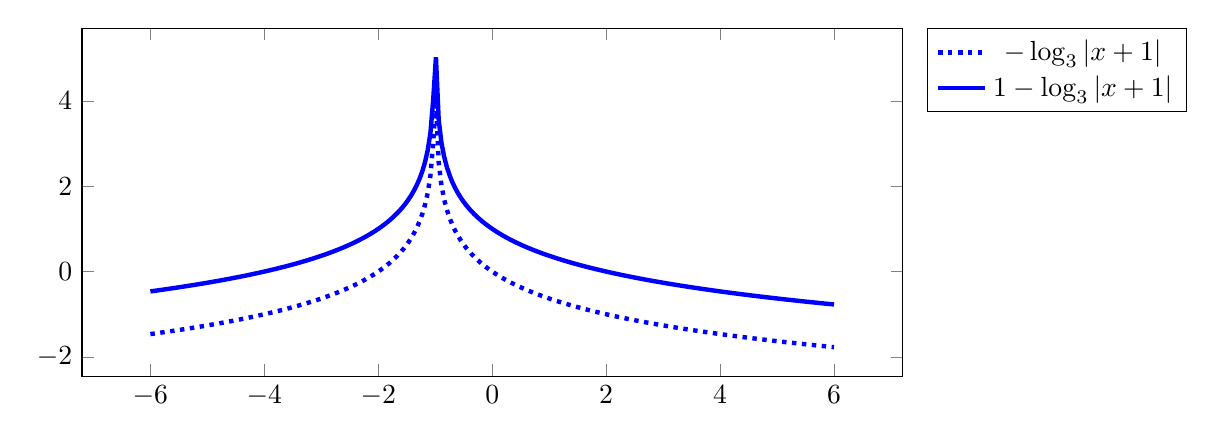
\begin{tikzpicture}
	\begin{axis}[width=12cm, height=6cm, samples=250, domain=-6:6,legend pos=outer north east]
	\addplot[blue, dotted, ultra thick]{-ln(abs(x+1))/ln(3)};
	\addlegendentry{$-\log_3{|x+1|}$}	
	\addplot[blue, ultra thick]{1-ln(abs(x+1))/ln(3)};
	\addlegendentry{$1-\log_3{|x+1|}$}	
	\end{axis}
	\end{tikzpicture}
\end{center}

% ---------------- Problem 3г----------------
Последовательность элементарных преобразований графика функции 3(г).
\begin{center}
	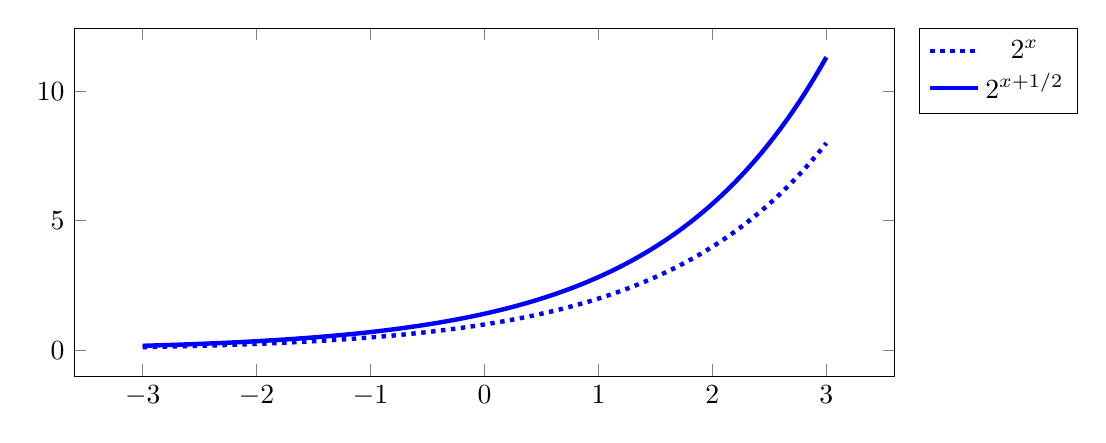
\begin{tikzpicture}
	\begin{axis}[width=12cm, height=6cm, samples=250, domain=-3:3,legend pos=outer north east]
	\addplot[blue, dotted, ultra thick]{2^x};
	\addlegendentry{$2^x$}	
	\addplot[blue, ultra thick]{2^(x+1/2)};
	\addlegendentry{$2^{x+1/2}$}	
	\end{axis}
	\end{tikzpicture}
	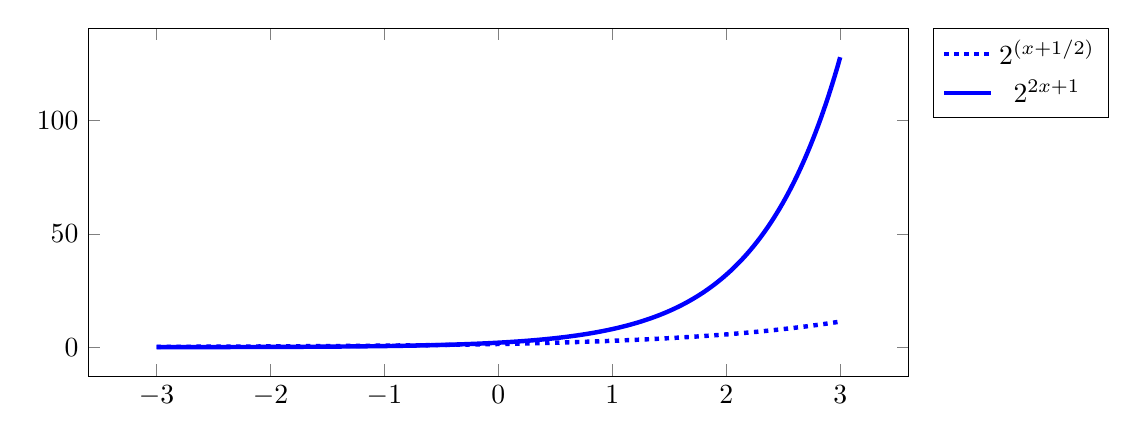
\begin{tikzpicture}
	\begin{axis}[width=12cm, height=6cm, samples=250, domain=-3:3,legend pos=outer north east]
	\addplot[blue,dotted, ultra thick]{2^(x+1/2)};
	\addlegendentry{$2^{(x+1/2)}$}	
	\addplot[blue, ultra thick]{2^(2*x+1)};
	\addlegendentry{$2^{2x+1}$}	
	\end{axis}
	\end{tikzpicture}
	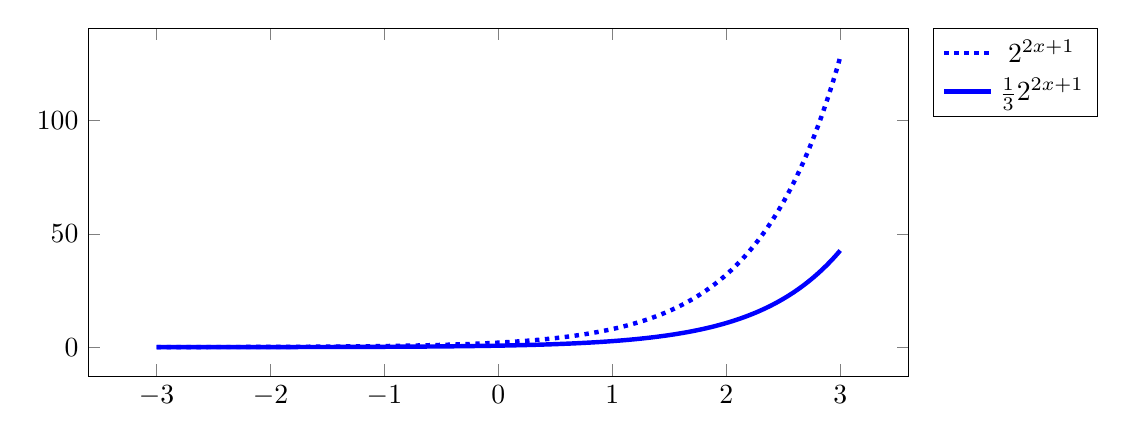
\begin{tikzpicture}
	\begin{axis}[width=12cm, height=6cm, samples=250, domain=-3:3,legend pos=outer north east]
	\addplot[blue, dotted, ultra thick]{2^(2*x+1)};
	\addlegendentry{$2^{2x+1}$}	
	\addplot[blue, ultra thick]{(1/3)*2^(2*x+1)};
	\addlegendentry{$\frac{1}{3}2^{2x+1}$}	
	\end{axis}
	\end{tikzpicture}
	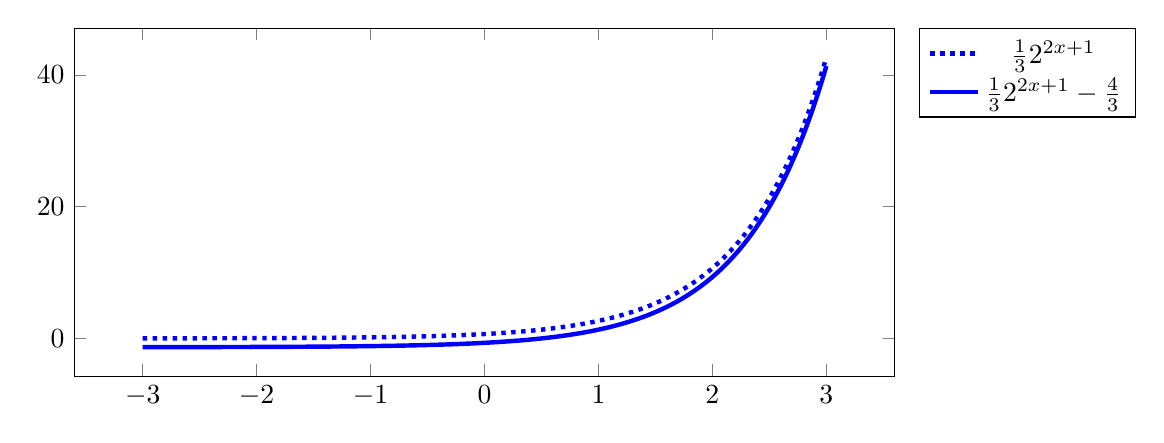
\begin{tikzpicture}
	\begin{axis}[width=12cm, height=6cm, samples=250, domain=-3:3,legend pos=outer north east]
	\addplot[blue, dotted, ultra thick]{(1/3)*2^(2*x+1)};
	\addlegendentry{$\frac{1}{3}2^{2x+1}$}	
	\addplot[blue, ultra thick]{(1/3)*2^(2*x+1)-(4/3)};
	\addlegendentry{$\frac{1}{3}2^{2x+1}-\frac43$}	
	\end{axis}
	\end{tikzpicture}
\end{center}

% ---------------- Problem 3д----------------
Последовательность элементарных преобразований графика функции 3(д).
\begin{center}
	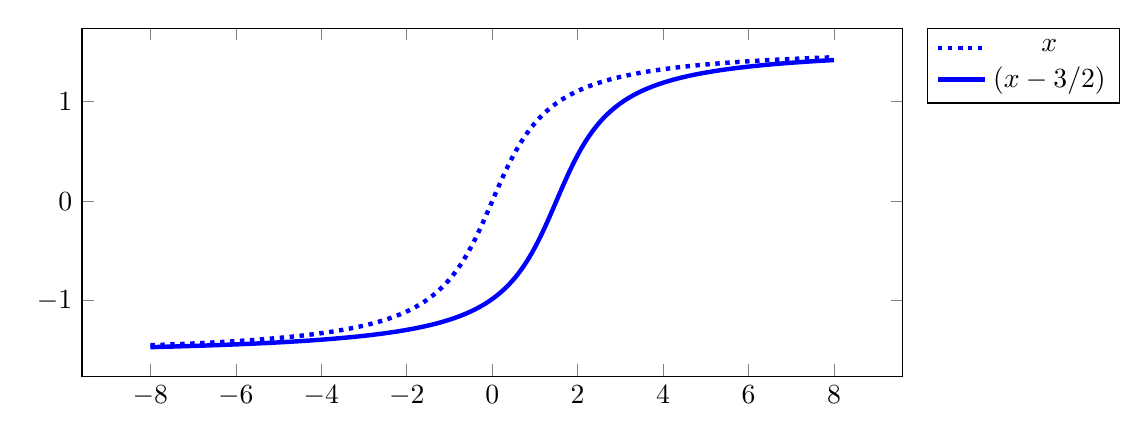
\begin{tikzpicture}
	\begin{axis}[width=12cm, height=6cm, samples=250, domain=-8:8,legend pos=outer north east]
	\addplot[blue, dotted, ultra thick]{rad(atan(x))};
	\addlegendentry{$\arctg{x}$}	
	\addplot[blue, ultra thick]{rad(atan(x-3/2))};
	\addlegendentry{$\arctg(x-3/2)$}	
	\end{axis}
	\end{tikzpicture}
	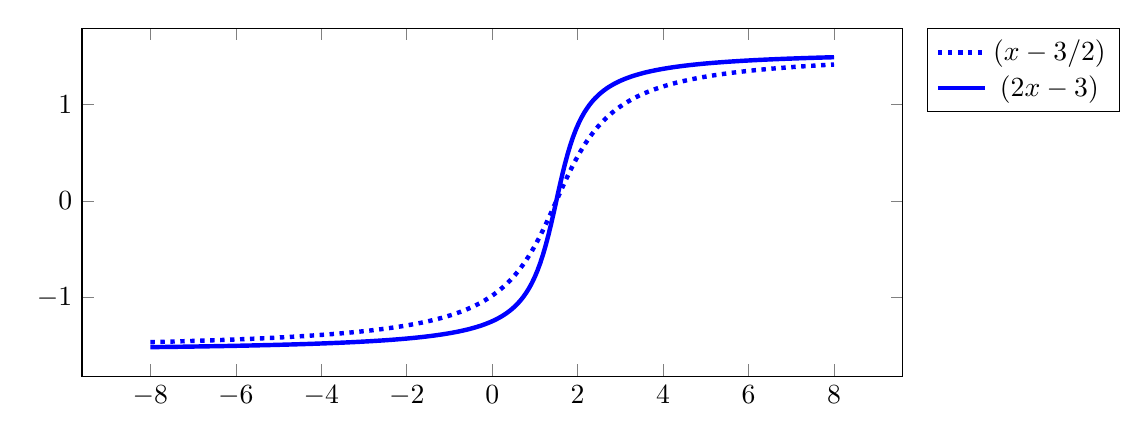
\begin{tikzpicture}
	\begin{axis}[width=12cm, height=6cm, samples=250, domain=-8:8,legend pos=outer north east]
	\addplot[blue, dotted, ultra thick]{rad(atan(x-3/2))};
	\addlegendentry{$\arctg{(x-3/2)}$}	
	\addplot[blue, ultra thick]{rad(atan(2*x-3))};
	\addlegendentry{$\arctg(2x-3)$}	
	\end{axis}
	\end{tikzpicture}
	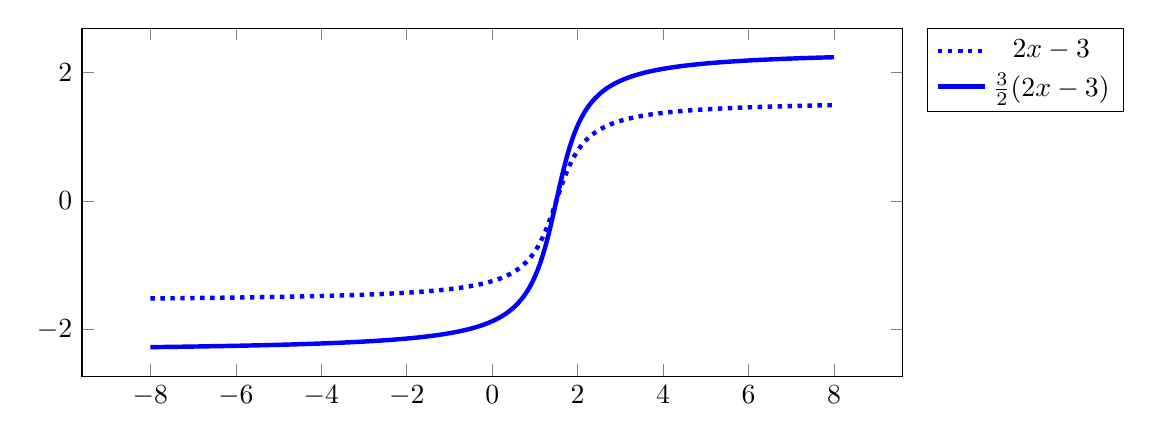
\begin{tikzpicture}
	\begin{axis}[width=12cm, height=6cm, samples=250, domain=-8:8,legend pos=outer north east]
	\addplot[blue, dotted, ultra thick]{rad(atan(2*x-3))};
	\addlegendentry{$\arctg{2x-3}$}	
	\addplot[blue, ultra thick]{1.5*rad(atan(2*x-3))};
	\addlegendentry{$\frac32\arctg(2x-3)$}	
	\end{axis}
	\end{tikzpicture}
	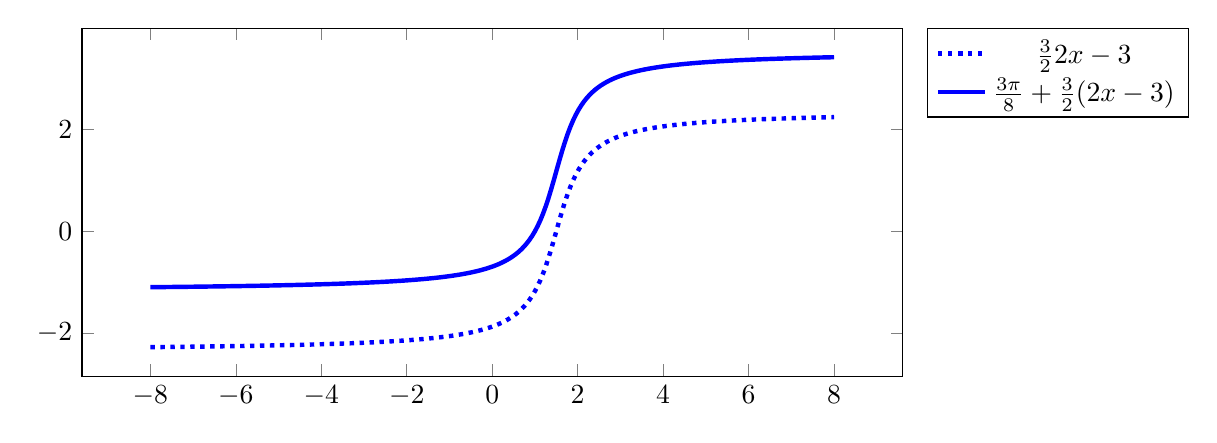
\begin{tikzpicture}
	\begin{axis}[width=12cm, height=6cm, samples=250, domain=-8:8,legend pos=outer north east]
	\addplot[blue, dotted, ultra thick]{1.5*rad(atan(2*x-3))};
	\addlegendentry{$\frac32\arctg{2x-3}$}	
	\addplot[blue, ultra thick]{(3*pi/8) + 1.5*rad(atan(2*x-3))};
	\addlegendentry{$\frac{3\pi}{8} + \frac32\arctg(2x-3)$}	
	\end{axis}
	\end{tikzpicture}
\end{center}

% ---------------------------- Problem 4----------------------------------
\subsubsection*{\center Задача № 4.}
{\bf Условие.~}
Построить эскиз графика рациональной функции, найдя его асимптоты и исследуя 
расположение графика относительно оси абсцисс и асимптот (не используя предела)
$$
y(x) = \dfrac{2x^2-x-3}{x^2-4x+4}.
$$
{\bf Решение.~}	
Выделим целую часть
$$
y(x) = \dfrac{2x^2-x-3}{x^2-4x+4} = \dfrac{2x^2-8x+8+7x-11}{(x-2)^2} = \dfrac{2(x-2)^2+7x-11}{x^2-4x+4} =
2 + \dfrac{7x-11}{(x-2)^2} .
$$
Отсюда, $y = 2$ --- горизонтальная ассимптота, а также, $x = 2$ --- вертикальная ассимптота.
\begin{center}
	\begin{tikzpicture}
	\begin{axis}[
	width=12cm, height=12cm,
	axis lines = center,
	xlabel = $x$,
	ylabel = {$y$},
	xmax = {8.5},
	xmin = {-5.5},
	ymax = {10.5},
	ymin = {-4.5},
	restrict y to domain = -5:10,
	legend pos = outer north east
	]
	\addplot [
	domain=-5:8,
	samples=500,
	color=black,
	ultra thick
	]
	{(2*x^2-x-3)/(x^2-4*x+4)};
	%\addlegendentry{2 turning points}
	
	% Oblique asymptote at y=x
	\addplot[dashed] {2};
	% Vertical asymptote at x=2
	\draw[dashed] ({axis cs:2,0}|-{rel axis cs:0,0}) -- ({axis cs:2,0}|-{rel axis cs:0,1});
	\end{axis}
	\end{tikzpicture}
\end{center}

% ---------------------------- Problem 5----------------------------------
\subsubsection*{\center Задача № 5.}
{\bf Условие.~}
Построить эскиз графика сложной функции, используя различные элементарные приёмы
$$
y(x) = \biggl(\dfrac{3}{2}\biggr)^x\cdot\cos\biggl(\dfrac{\pi x}{2}\biggr).
$$
{\bf Решение.~}	График функции $y(x)=\cos(\pi x/2)$ получается элементарными преобразованиями из
графика функции $y(x)=\cos(x)$. В то же время, график функции $y(x)=(3/2)^x\cos(\pi x/2)$ получается
из графика функции $y(x)=\cos(\pi x/2)$  пропорциональным изменением ординаты каждой точки графика в $(3/2)^x$ раз для
каждого значения абсциссы $x$.
\begin{center}
	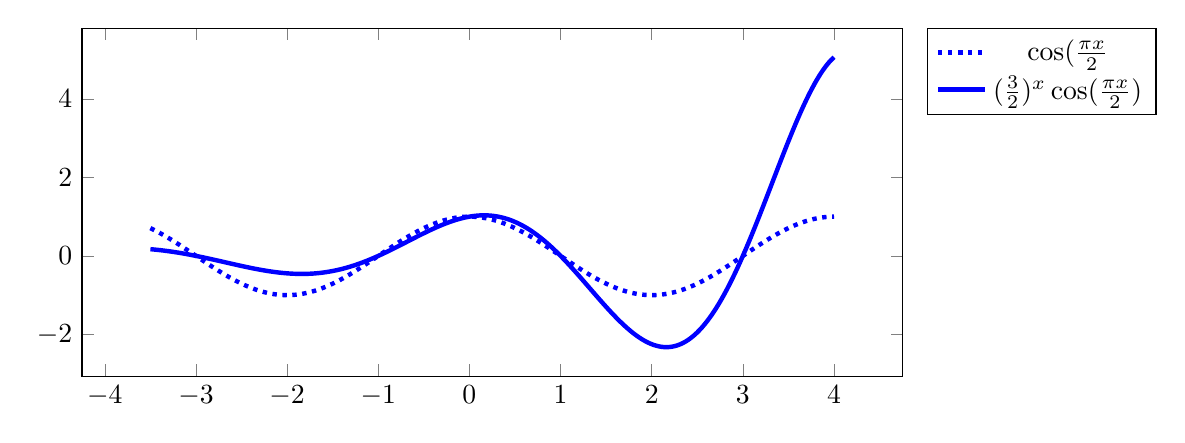
\begin{tikzpicture}
	\begin{axis}[width=12cm, height=6cm, samples=250, domain=-3.5:4,legend pos=outer north east]
	\addplot[blue, dotted, ultra thick, samples=250, domain=-3.5:4]{cos(deg(0.5*pi*x))};
	\addlegendentry{$\cos(\frac{\pi x}{2}$}
	\addplot[blue, ultra thick, samples=250, domain=-3.5:4]{((1.5)^x)*cos(deg(0.5*pi*x))};
	\addlegendentry{$(\frac32)^x\cos(\frac{\pi x}{2})$}
	\end{axis}
	\end{tikzpicture}
\end{center}